\documentclass[a4paper]{article}

\usepackage{algorithm,amsmath}
\usepackage[pdftex]{graphicx}
\usepackage[margin=3.5cm]{geometry}
\usepackage[format=hang,labelfont=it]{caption}
\usepackage[noend]{algorithmic}

\floatname{algorithm}{Listing}

\begin{document}

\title{
  {\small
    Halmstad University course DA4002\\
    Introduction to Algorithms, Data Structures, and Problem Solving\\
  }
  Group Activities for Lecture 7
}
\maketitle



\section{Topological Ordering}

\emph{This group activity is based on question~6 of the written exam from October, 2011.}

\paragraph{Definition:}
A \textbf{topological ordering} of a directed graph is a sequence of its vertices such that, for every edge $(u,v)$, $u$ appears before $v$ in the sequence.
Note that for any path from $u$ to $v$, this also implies that $u$ comes before $v$ in the ordering.
In the example graph shown below, the sequence $(C,A,D,B)$ is a topological ordering.

\begin{center}
  \fbox{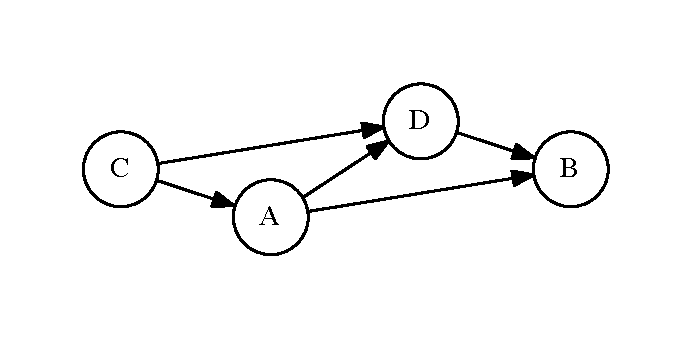
\includegraphics[width=0.3\columnwidth,trim=1cm 1cm 1cm 1cm]{dag-small.pdf}}
\end{center}

\paragraph{Theorem:}
A topological ordering is possible if and only if the graph has no cycles.
In other words, a graph has to be a \textbf{directed acyclic graph} (DAG) in order to have a topological ordering.
And also, every DAG has at least one topological ordering.

\begin{enumerate}
\item
  The class is subdivided into two groups.
  Discuss how you can prove the theorem.
\item
  Each student individually should apply Kahn's Algorithm (shown in Listing~\ref{algo:kahn}) to the two graphs in Figure~\ref{fig:graphs}.
  Then compare your results with someone else in your group.
\end{enumerate}

\begin{algorithm}
  \caption{Kahn's Algorithm}\label{algo:kahn}
  \begin{algorithmic}
    \REQUIRE a directed graph $G$
    \STATE $L \leftarrow$ initially empty list
    \STATE $S \leftarrow$ Set of all nodes that have \textbf{no incoming} edges
    \WHILE { $S \neq \emptyset$ }
      \STATE remove a node $n$ from $S$
      \STATE insert $n$ into $L$
      \FORALL { nodes $m$ with an edge $e = (n,m)$ }
        \STATE remove $e$ from $G$
        \IF { $m$ has not other incoming edge }
          \STATE insert $m$ into $S$
        \ENDIF
      \ENDFOR
    \ENDWHILE
    \IF { $G$ has edges }
      \RETURN error ``graph has at least one cycle''
    \ENDIF
    \RETURN $L$
  \end{algorithmic}
\end{algorithm}

\begin{figure}
  \centering
  \fbox{
    \begin{minipage}{0.35\columnwidth}
      \centering
      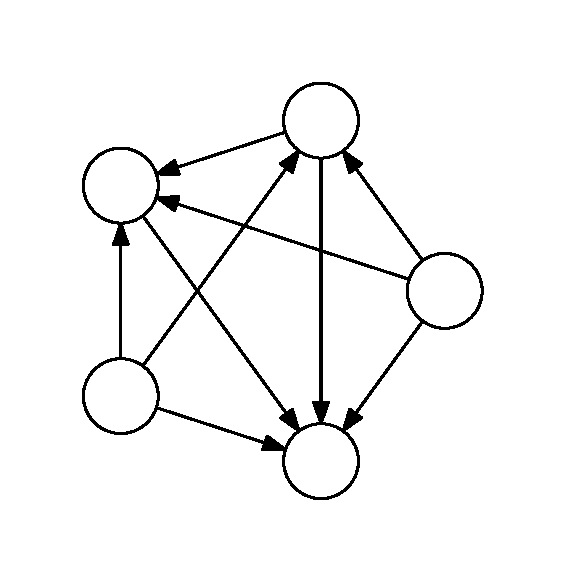
\includegraphics[width=\columnwidth,trim=1cm 1cm 1cm 1cm]{cycle-detection-dag.pdf}
      \textbf{graph A}
    \end{minipage}}
  \fbox{
    \begin{minipage}{0.35\columnwidth}
      \centering
      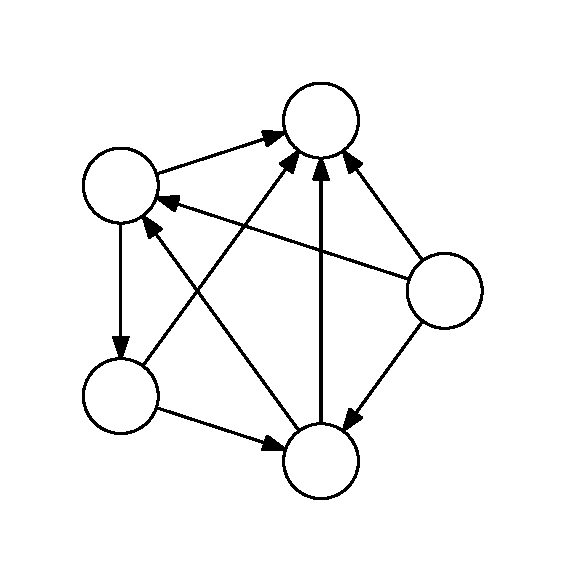
\includegraphics[width=\columnwidth,trim=1cm 1cm 1cm 1cm]{cycle-detection-non-dag.pdf}
      \textbf{graph B}
    \end{minipage}}
  \caption{Example graphs for topological ordering}\label{fig:graphs}
\end{figure}


\end{document}
